\documentclass[conference]{IEEEtran}
\IEEEoverridecommandlockouts
% The preceding line is only needed to identify funding in the first footnote. If that is unneeded, please comment it out.
%Template version as of 6/27/2024

\usepackage{cite}
\usepackage{amsmath,amssymb,amsfonts}
\usepackage{algorithmic}
\usepackage{graphicx}
\usepackage{textcomp}
\usepackage{xcolor}
\usepackage{makecell}
\def\BibTeX{{\rm B\kern-.05em{\sc i\kern-.025em b}\kern-.08em
    T\kern-.1667em\lower.7ex\hbox{E}\kern-.125emX}}
\begin{document}
\pagestyle{plain}
\pagenumbering{arabic} % Sets page numbering to arabic (1, 2, 3, ...)
\setcounter{page}{1} % Specifies the starting page number

% fix for unaligned author blocks
% from https://tex.stackexchange.com/questions/458204/ieeetran-document-class-how-to-align-five-authors-properly/458208#458208

\makeatletter
\newcommand{\linebreakand}{%
    \end{@IEEEauthorhalign}
    \hfill\mbox{}\par
    \mbox{}\hfill\begin{@IEEEauthorhalign}
}
\makeatother

\title{Evolutionary Hyperparameter Optimization to Find Lightweight CNN Models for Autonomous Steering}

\author{\IEEEauthorblockN{Devson Butani}
    \IEEEauthorblockA{\textit{Department of Math and Computer Science} \\
        \textit{Lawrence Technological University}\\
        Southfield, MI, USA \\
        dbutani@ltu.edu}
    \and
    \IEEEauthorblockN{Ryan Kaddis}
    \IEEEauthorblockA{\textit{Department of Math and Computer Science} \\
        \textit{Lawrence Technological University}\\
        Southfield, MI, USA \\
        rkaddis@ltu.edu}
    \linebreakand
    \IEEEauthorblockN{Giuseppe DeRose Jr.}
    \IEEEauthorblockA{\textit{Department of Math and Computer Science} \\
        \textit{Lawrence Technological University}\\
        Southfield, MI, USA \\
        gderose@ltu.edu}

    \and
    \IEEEauthorblockN{Chan-Jin Chung}
    \IEEEauthorblockA{\textit{Department of Math and Computer Science} \\
        \textit{Lawrence Technological University}\\
        Southfield, MI, USA \\
        cchung@ltu.edu}
}

\maketitle

\begin{abstract}
    This research investigates the optimization of Convolutional Neural Networks (CNNs) for autonomous steering using the (N+M) Evolutionary Strategy (ES) with the 1/5th success rule. The primary objective is to develop a lightweight CNN model capable of real-time steering angle prediction, mimicking human driving behavior on predefined paths. The ES algorithm automates hyperparameter tuning, dynamically adjusting parameters such as filter sizes and layer configurations. Data collection encompasses driving scenarios recorded via the LTU ACTor autonomous driving platform, including variations in path direction and driving style. The dataset consists of timestamped images labeled with steering angles, pre-processed to focus on relevant visual information. Initial experiments involve training a baseline CNN model, which is then refined using ES to significantly reduce model size while maintaining competitive predictive accuracy. The results highlight the viability of lightweight CNN architectures for real-time autonomous systems, striking a balance between computational efficiency and performance. This study not only advances research initiatives in using evolutionary strategies for autonomous driving applications but also lays the groundwork for deploying cost-effective, scalable solutions in self-driving technology.
\end{abstract}

\begin{IEEEkeywords}
    Evolutionary Strategy, Hyperparameter Optimization, Convolutional Neural Networks (CNN), Lightweight CNN, Autonomous Driving, Deep Learning, Real-Time Performance, Autonomous Vehicles, Cameras
\end{IEEEkeywords}

\section{Introduction}
Autonomous driving systems require robust models capable of making real-time decisions under varying conditions. A critical component of these systems is the prediction of steering angles based on camera input, which involves processing visual data effectively and efficiently on compute-limited on-board processors~\cite{PilotNET_application}. This research focuses on training and optimizing CNNs leveraging evolutionary strategies (ES) to automate the search for the best-performing and best size-reduced model configurations.

This research directly addresses the limitations that come with larger models and limited data. Larger models, while often achieving higher accuracy, come with increased computational cost and memory requirements, which can lead to slower inference times and higher energy consumption~\cite{self_drive_latency_and_model_size_drawbacks}. This poses a significant challenge for real-time applications like autonomous driving, where split-second decisions and energy efficiency are crucial. The size of a model directly impacts its deployment feasibility, particularly in resource-constrained on-board processors~\cite{MobileNET_size_and_speed}. Minimizing model size while also training with limited data is the core design challenge in autonomous driving systems.

Furthermore, the performance of deep learning models is heavily reliant on the availability of large, diverse, and labeled datasets. In the context of autonomous driving, collecting and annotating such datasets for every conceivable scenario is impractical and cost-prohibitive~\cite{ImageNET_large_scale_database} Even though limited data can lead to overfitting, where the model performs well on the training data but fails to generalize to unseen scenarios or conditions, this is often not a problem in real-world applications where the operational design domain (i.e., the area of interest) can be regulated. For example, deploying an autonomous vehicle specifically for a small city or a specific set of routes. With this method, we can leverage adding small datasets everyime the domain expands and utilize techniques like transfer learning and few shot learning to improve model performance over time~\cite{few_shot_learning}. While optimization techniques have been extensively explored in various domains, their application to creating lightweight and adaptable models for autonomous driving, specifically for real-time steering angle prediction, remains an active area of research.

Evolutionary Strategies (ES) offer a compelling advantage in this context. ES is a population-based optimization algorithm that leverages the collective intelligence of a population of candidate solutions to find the best-performing solution within a given search space~\cite{ES_introduction}. Unlike gradient-based optimization methods, which can struggle in complex, non-differentiable, or noisy search spaces, ES algorithms are well-suited for exploring such landscapes~\cite{ES_scalable}. This is particularly relevant to hyperparameter optimization of CNNs for autonomous driving, where the relationship between model architecture, hyperparameters, and performance can be highly complex and non-linear.

\subsection{Data Acquisition and Preprocessing}

\textbf{Equipment:} The LTU ACTor autonomous driving platform, integrated with the Robot Operating System (ROS), was used for data collection. Sensor data, including images from the vehicle's forward-facing camera and corresponding steering angles, were recorded in rosbag files. This setup ensured synchronized visual and control data, essential for training and evaluating the models.

\textbf{Environment:} Data was collected along a predefined circular path: the red brick path surrounding Ockham's Wedge at LTU. To introduce variability and enhance model robustness, driving sessions included clockwise and counterclockwise directions, smooth and zigzag maneuvers, and driving along inner and outer path edges to simulate diverse spatial alignments.  Figure~\ref{fig:ockham} shows an overhead view of the data collection site.

\begin{figure}[ht]
    \centering
    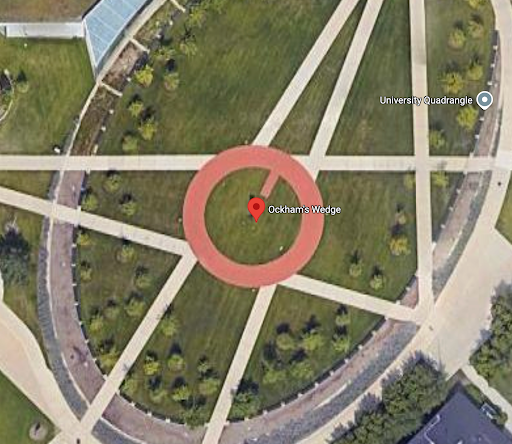
\includegraphics[width=2.2in]{assets/circle-maps.png}
    \caption{ Aerial view of Ockham's Wedge at Lawrence Technological University. Data was collected from the red brick circle surrounding the art piece. }
    \label{fig:ockham}
\end{figure}

\textbf{Extraction and Preprocessing:} A custom script was developed to extract and preprocess data from rosbag files.

\begin{figure}[ht]
    \centering
    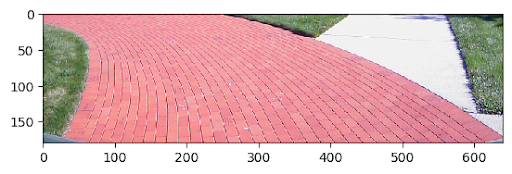
\includegraphics[width=2.5in]{assets/leftturn.png}
    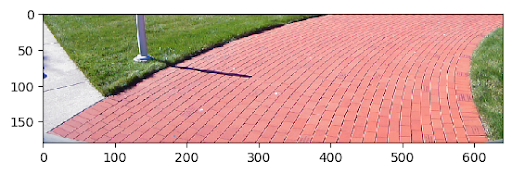
\includegraphics[width=2.5in]{assets/rightturn.png}
    \caption{Sample images after cropping and preprocessing. The extracted steering angles are 12.901 degrees (Top) and -10.099 degrees (Bottom).}
    \label{fig:preprocessed_images}
\end{figure}

Images were saved at 200 ms intervals, with filenames encoding timestamps and steering angles. Each image was cropped to exclude irrelevant regions, such as the sky and surrounding buildings. The resulting dataset consisted of 2,957 images, split into 70\% training (2,069), 20\% validation (592), and 10\% testing (296). Even though the dataset is small, it is representative of real-world driving scenarios and provides a useful benchmark for evaluating model performance.

\subsection{Research Goals}

Since there are many experiments in image to steering angle prediction that have shown quaility improvements over the years~\cite{PilotNET_application,lane_detection_good_results_zigzag,CNN_can_self_drive}, the proposed ES based optimization should allow for a significant improvement in deployable performance and ability to run real-time inference on on-board compute resources. The primary goals of this research are to:

\begin{enumerate}
    \item Develop a framework to apply the (N+M) Evolutionary Strategy (ES) with the 1/5th success rule for automated hyperparameter tuning.
    \item Minimize the size of the baseline CNN model while maintaining satisfactory steering angle prediction performance.
    \item Validate the real-world applicability of ES-optimized models in autonomous vehicle systems.
\end{enumerate}

\section{Methodology}

\subsection{Model Training and Baseline Establishment}

Models are trained using the Keras API with a PyTorch backend to leverage GPU compute capacity. The training process employs the Mean Squared Error (MSE) loss function, which quantifies the average squared difference between predicted and actual steering angles. The Mean Absolute Error (MAE) serves as a key performance metric, indicating the average deviation in steering angle predictions in degrees. This provides a straightforward and interpretable measure of model accuracy for autonomous steering applications. Minimizing both MSE and MAE is crucial for achieving precise control of the vehicle. These metrics serve as benchmarks for evaluating the efficacy of the Evolutionary Strategy (ES) with the 1/5 success rule in optimizing model architectures.

Initial experiments began with a single-layer CNN to establish a rudimentary baseline. However, the limited capacity of this architecture quickly became apparent, rendering it unsuitable for real-world driving scenarios. To address this, the PilotNET architecture, a CNN developed by NVIDIA~\cite{PilotNET} was adopted. PilotNET, an early milestone in autonomous steering research, demonstrated the potential of GPU-accelerated deep learning for this domain. Leveraging a proven architecture allowed for a more effective comparison of ES-optimized models against a recognized standard.

To enhance training efficiency and prevent over optimization, early stopping was implemented. Training instances are terminated if no improvement in the MSE metric is observed after four epochs. This strategy prevents the allocation of computational resources to hyperparameters that do not contribute to model performance, thereby accelerating the optimization process.

\subsection{Hyperparameter Management}

Initially, the hyperparameter space included individual layer units (number of filters in convolutional layers and neurons in fully connected layers), batch sizes, learning rates, activation functions, and optimizer selection. To facilitate a comprehensive exploration of potential architectures, layer units were allowed to vary from 20\% to 300\% of the PilotNet baseline.

\begin{table}[ht]
    \centering
    \caption{Hyperparameter Search Spaces}
    \begin{tabular}{l|r}
        \textbf{Hyperparameter} & \textbf{Search Space}     \\
        \hline
        Layer Units             & 20\% to 300\% of PilotNet \\
        Batch Size              & 1 - 32                    \\
        Learning Rate           & 0.001 - 1.5               \\
        Activation Function     & ReLU, eLU, Sigmoid, Tanh  \\
        Optimizer               & Adam, SGD, RMSprop        \\
    \end{tabular}
    \label{tab:searchspace}
\end{table}

However, preliminary experiments indicated that focusing the optimization efforts solely on layer units resulted in improved performance and reduced search time significantly. Consequently, batch size (32), learning rate (0.001), activation function (ReLU), and optimizer (Adam) were fixed to match the baseline model settings. This narrowed scope then allowed the Evolutionary Strategy (ES) to concentrate on the most impactful architectural parameters, leading to more efficient exploration of the design space. The ranges of the layer units explored are provided in Table~\ref{tab:searchspace}.

\subsection{Optimization Framework}

CNN hyperparameters, specifically the number of filters in convolutional layers and the number of neurons in fully connected layers, are encoded as genes within an Evolutionary Strategy (ES) framework. The (N+M)-ES approach is employed, iteratively optimizing hyperparameters by combining the N best-performing parent models with M offspring models generated through mutation. This approach allows for both exploitation of promising regions of the hyperparameter space (through selection of top parents) and exploration of new possibilities (through mutation of offspring).

\subsection{ES Algorithm}

The Evolutionary Strategy (ES) optimization process unfolds as follows:

\begin{enumerate}
    \item \textbf{Initialization:} Generate and train N parent models with random hyperparameters sampled within predefined ranges. The initial hyperparameters are drawn from a uniform distribution within the specified ranges. The number of parents, N, is a tunable parameter that controls the diversity of the population.
    \item \textbf{Child Generation:} Create M offspring by mutating parent hyperparameters according to the following equation:

          \begin{equation}
              \hat{h} = h + \text{gauss}(\sigma * (\text{max}(h) - \text{min}(h)))
          \end{equation}

          where \(\hat{h}\) represents the mutated hyperparameter value. \(h\) is the original hyperparameter value from the parent model. \(\text{gauss}(\mu, \sigma)\) is a random number drawn from a Gaussian distribution with mean \(\mu\) and standard deviation \(\sigma\).  In this case, \(\mu = 0\). \(\sigma\) is the mutation step size, controlling the magnitude of the mutation. \(\text{max}(h)\) and \(\text{min}(h)\) define the upper and lower bounds of the hyperparameter search space, respectively.

          The term \((\text{max}(h) - \text{min}(h))\) normalizes the mutation step size to the range of the hyperparameter, ensuring that the mutation is proportional to the scale of the parameter.
    \item \textbf{Training and Evaluation:} Train all offspring models and evaluate their performance based on validation loss (MSE) and accuracy (MAE).
    \item \textbf{Selection:} Retain the top N models (from parents and children) based on validation performance to form the next generation's parent population. This selection process ensures that the most promising models are carried forward, driving the evolution towards improved performance. The mutation step size (\(\sigma\)) is dynamically adjusted using the 1/5 success rule~\cite{ES_one_fifth_rule}:

          \begin{equation}
              \sigma_{t+1} = \left\{
              \begin{array}{ll}
                  \alpha * \sigma_t & \text{success rate} > \frac{1}{5} \smallbreak \\
                  \beta * \sigma_t  & \text{success rate} \leq \frac{1}{5}          \\
              \end{array}
              \right.
          \end{equation}

          where \(\sigma_{t+1}\) is the updated step size for the next generation. \(\sigma_t\) is the current step size. \(\alpha > 1\) is a scaling factor to increase the step size (e.g., 1.1). \(\beta < 1\) is a scaling factor to decrease the step size (e.g., 0.9). The "success rate" is defined as the fraction of offspring that outperform their parents in terms of validation performance.

          ~~If the success rate is greater than 1/5, the step size is increased, encouraging greater exploration of the hyperparameter space. Conversely, if the success rate is less than or equal to 1/5, the step size is decreased, promoting more focused refinement of promising solutions. This adaptive mechanism ensures efficient exploration while avoiding premature convergence to local optima.

\end{enumerate}

\textbf{Computational Resources: } Training is performed on Lawrence Technological University's NVIDIA A100 GPU server, enabling efficient parallel training of N parent and M offspring model pools. The large VRAM capacity of the A100 GPU allows for the use of larger N and M values, which increases the diversity of the population and enhances the exploration of the hyperparameter space. The specific values of N and M are determined based on the available computational resources and the complexity of the optimization problem.

\subsection{Model Selection}

Four different model architectures are proposed for determining the effect of ES on model performance and size. The first model, named "Baseline", is the same architecture established by PilotNET.~\cite{PilotNET} The second model, named "Optimized", contains a CNN and DNN structure that has been optimized with ES, within the search space proposed by Table~\ref{tab:searchspace}. The third model, named "Half-Size", contains the PilotNET CNN architecture with half of the baseline number of neurons per layer, and half of the search space proposed by Table~\ref{tab:searchspace}. The fourth model, named "Quarter-Size", contains the PilotNET CNN architecture with a quarter of the baseline number of neurons per layer, and a quarter of the search space proposed by Table~\ref{tab:searchspace}. These four models allow the effect of ES on model performance with smaller model sizes to be observed.

\begin{table}[ht]
    \centering
    \caption{Model Descriptions}
    \begin{tabular}{p{0.75in}|p{2.25in}}

        \textbf{Model Name} & \textbf{Description}                                                 \\
        \hline
        Baseline            & PilotNET architecture, baseline for comparison.                      \\
        % \hline
        Optimized           & ES-optimized CNN \& DNN layers.                                      \\
        % \hline
        Half-Size           & Half the size of baseline CNN layers and ES-optimized DNN layers.    \\
        % \hline
        Quarter-Size        & Quarter the size of baseline CNN layers and ES-optimized DNN layers. \\
    \end{tabular}
    \label{tab:aliases}
\end{table}

\subsection{Model Testing}

To validate the real-time applicability of the ES-optimized models, a series of tests were conducted within a 2D simulation environment, GazelleSim~\cite{gazelle_sim}. The simulation allows for controlled and repeatable testing of the steering control algorithms on the red brick circular path used for training. This serves as the operational design domain for our ES-optimized models.

\begin{figure}[ht]
    \centering
    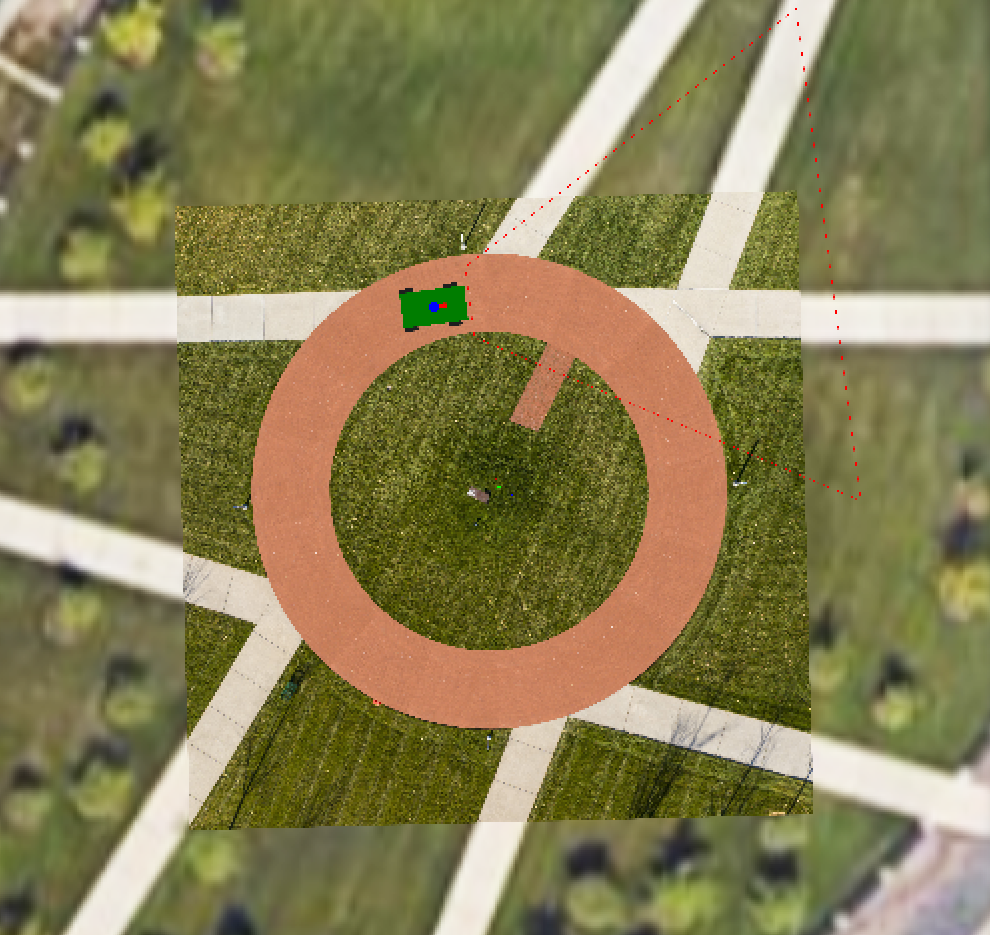
\includegraphics[width=3in]{assets/Gazelle-Playing-Field.png}
    \caption{ Aerial vi w of the playing field in the GazelleSim environment.}
    \label{fig:field}
\end{figure}

The autonomous driving testing pipeline operates as follows:

\begin{enumerate}
    \item \textbf{Image Acquisition:} Simulated camera images are captured from the 2D environment, representing the vehicle's forward view.
    \item \textbf{Model Inference:} The captured image is fed into the trained model, which predicts a steering angle. The predicteed steering angle represents the desired direction of the vehicle.
    \item \textbf{Steering Control:} The predicted steering angle is then translated into a control command that adjusts the vehicle's trajectory within the simulation. The steering angle is converted into a control signal that influences the vehicle's direction and speed. For real-world testing, this control signal is sent to the real vehicle's steering and throttle actuators instead.
    \item \textbf{Closed-Loop Feedback:} This whole process creates a closed-loop control system that runs in real-time.
\end{enumerate}

\begin{figure}[ht]
    \centering
    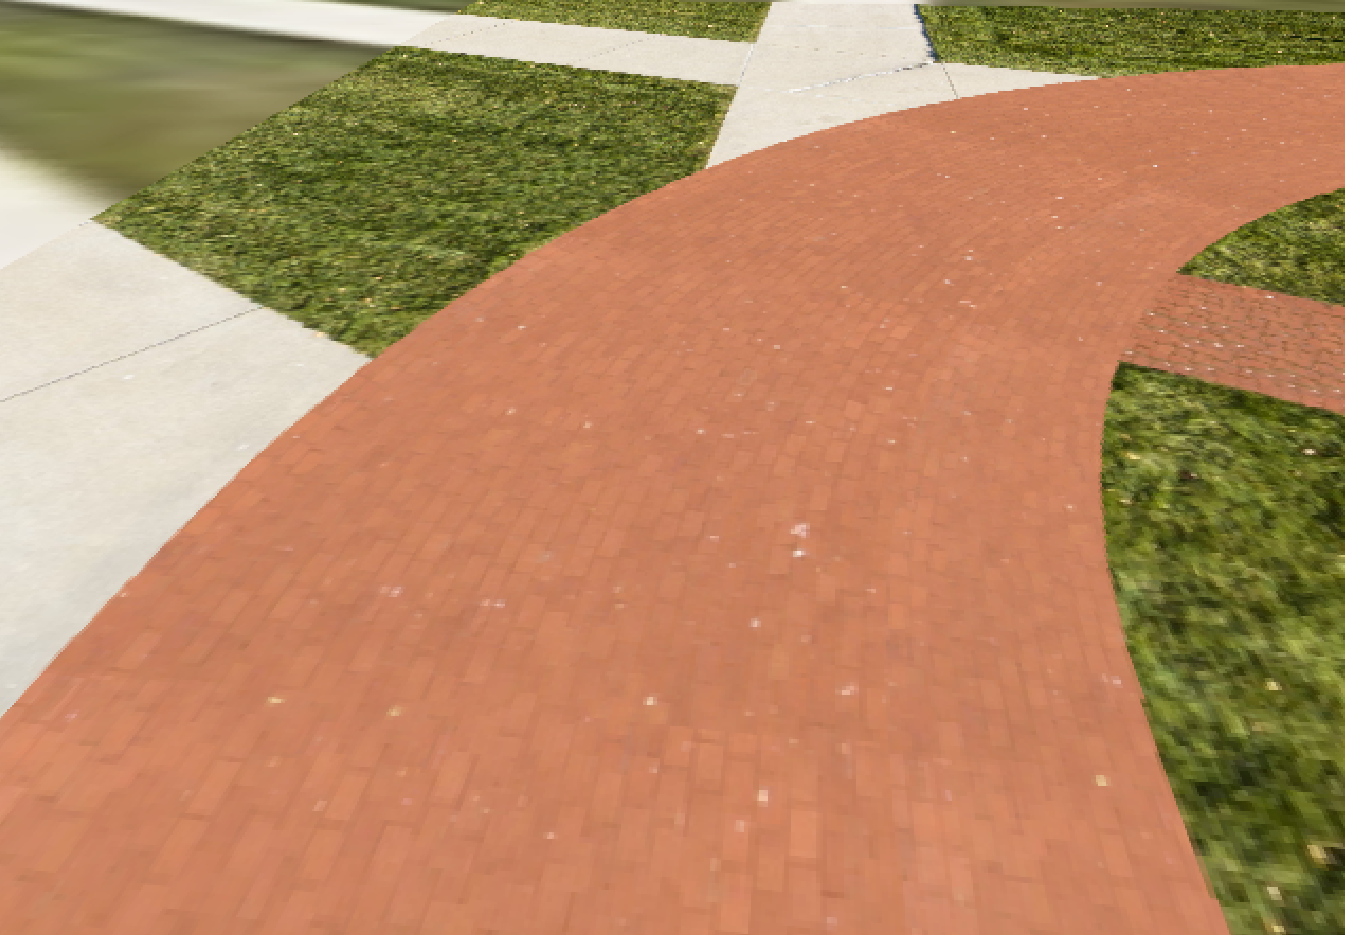
\includegraphics[width=3in]{assets/Gazelle-Camera-View.png}
    \caption{ Perspective view of the playing field from the GazelleSim vehicle. }
    \label{fig:camview}
\end{figure}

\section{Experimental Results}

Table~\ref{tab:testarch} presents the neurons per layer of each of the four trained and optimized models. Bolded layers are optimized using ES.

\newcommand{\gr}{\textgreater}

\begin{table}[ht]
    \centering
    \caption{ES-Optimized Model Architectures}
    \begin{tabular}{c|c}

        \textbf{Model} & \textbf{Architecture}                                       \\
        \hline
        Baseline       & \makecell[l]{CNN: 24 \gr 36 \gr 48 \gr 64 \gr 64 \gr        \\
        DNN: 1164 \gr 100 \gr 50 \gr 10 \gr 1}                                       \\
        \hline
        Optimized      & \makecell[l]{\textbf{CNN: 6 \gr 9 \gr 43 \gr 28 \gr 61 \gr} \\
        \textbf{DNN: 2328 \gr 146 \gr 100 \gr 20} \gr 1}                             \\
        \hline
        Half-Size      & \makecell[l]{CNN: 12 \gr 18 \gr 24 \gr 32 \gr 32 \gr        \\
        \textbf{DNN: 149 \gr 14 \gr 20} \gr 1}                                       \\
        \hline
        Quarter-Size   & \makecell[l]{CNN: 6 \gr 9 \gr 12 \gr 16 \gr 16 \gr          \\
        \textbf{DNN: 8 \gr 3} \gr 1}                                                 \\
    \end{tabular}
    \label{tab:testarch}
\end{table}

\begin{figure}[ht]
    \centering
    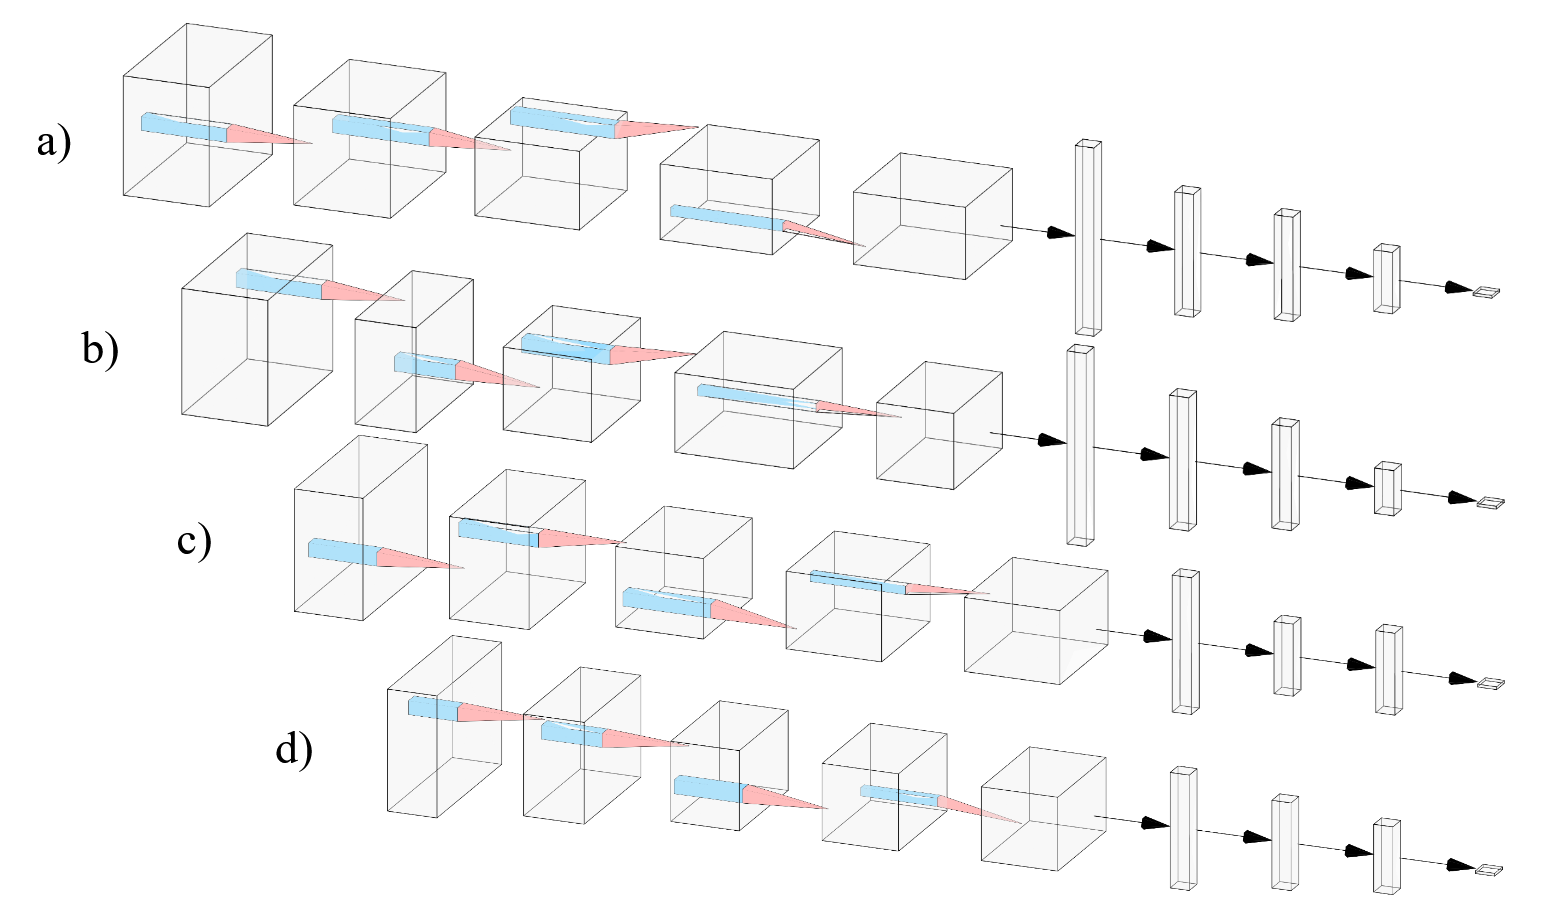
\includegraphics[width=3in]{assets/alexnet.png}
    \caption{ Visual representation of the models by layer. a) Baseline. b) Optimized. c) Half-Size. d) Quarter-Size. }
    \label{fig:alexnet}
\end{figure}

Table~\ref{tab:compute} details the performance and size metrics of each of the four models.

\begin{table}[ht!]
    \centering
    \caption{Compute Utilization}
    \begin{tabular}{c|c|c|c|c}

        \textbf{Model} & \textbf{Parameters} & \textbf{Memory (MB)} & \textbf{MSE} & \textbf{MAE} \\
        \hline
        Baseline       & 245M                & 936                  & 1.01         & 0.63         \\
        Optimized      & 250M                & 1050                 & 0.49         & 0.41         \\
        Half-Size      & 61.4M               & 420                  & 1.33         & 0.78         \\
        Quarter-Size   & 4.97M               & 146                  & 1.88         & 0.88         \\
    \end{tabular}
    \label{tab:compute}
\end{table}

\section{Discussion}
The results demonstrate the effectiveness of using evolutionary strategies (ES) with 1/5 success rule to optimize CNN architectures for steering angle prediction in autonomous driving systems and hence meets our goals. Key findings include:
Baseline Performance: The PilotNET baseline achieved reasonable accuracy but required significant computational resources due to its large model size (245.40 million parameters, 936.44 MB).
This highlights the need for architecture optimization to improve efficiency without sacrificing performance.
Impact of ES Optimization: The ES-optimized PilotNET model achieved the lowest error (MSE: 0.49, MAE: 0.41 degrees) while significantly reducing the model size (50.97 million parameters, 194.45 MB). Models with reduced convolutional layers showed trade-offs: while they consumed fewer resources, their prediction accuracy relatively suffered, with the quarter-size model exhibiting the highest error (MSE: 1.88, MAE: 0.88 degrees). This study shows that using ES to optimize models for better performance or size reduction while does yield practical results that can improve application efficiency.
Real-time Performance: Visual results confirm that the optimized models deliver accurate steering predictions even in complex driving scenarios, with low absolute errors between expected and predicted steering angles. In real-world applications a small difference in error (<1.0 degree) with a major difference in model size (5-25\% of baseline size) is a valid tradeoff.

In the future, we plan to:
\begin{enumerate}
    \item Expand the dataset by recording driving data on various roads across the LTU campus, including different surfaces, path geometries, and lighting conditions.
    \item Add Recurrent Neural Network layers to train models based on the past steering inputs.
    \item Deploy the optimized CNN models on the LTU ACTor autonomous driving platform.
    \item Evaluate optimized models on low-power compute platforms, such as NVIDIA Jetson or Raspberry Pi, to assess scalability for cost-effective systems.
\end{enumerate}

\clearpage
\bibliographystyle{plain} % We choose the "plain" reference style
\bibliography{references} % Entries are in the references.bib file

\end{document}